\vspace{-1em}
\section{Conclusion and Future Work}
\vspace{-0.75em}

We show that some of today's specialized applications have large, structured
namespaces and propose a new way for the file system to facilitate this
domain-specific knowledge.  By leveraging the bounded/balanced nature of these
namespaces, clients/servers can exchange compact representations of metadata
instead of the metadata in its entirety.  This work shares many of the risks of
programmable storage~\cite{sevilla:eurosys17-malacology, sevilla:sc15-mantle},
namely introducing poorly designed generators ({\it e.g.}, non-deterministic
naming) into the file system.  Proper sandboxing techniques for
security/correctness are future work.  Also, our generators may not work for
applications that make use of metadata that cannot be specified at create time,
such as permissions ({\it e.g}, workflows), size of the file ({\it e.g.},
Hadoop), or dates ({\it e.g.}, garbage collectors).  Another avenue of future
work will supplement these generators with more metadata information.

%  Namespace schemas and generators solve many file system mtadata
%read problems because clients and servers avoid exchanging large lists. 
%Our
%examples benefit from  \emph{metadata compaction}, which speeds up
%network/storage overheads and gives clients and servers the ability to
%\emph{modify large namespaces} and \emph{generate relevant parts of the
%namespace}.


%File systems are thought to
%be robust and general because they have been around for a long time. But we
%show that today's applications are specialized, so they have regular, large
%namespaces. As a result, the file system should be changing its internal
%mechanisms to leverage the bounded and balanced nature of these namespaces to
%optimize metadata performance.

%In this section, we show how clients and metadata servers communicate using the
%Pattern PLFS language and present our
%storage system that adapts to the wokload
%(Section~\ref{sec:adapting-to-the-workload-with-cudele})).  Other destructive
%solutions include changing the storage system and altering the application.
%
%\subsection{Adapting to the Workload with Cudele}
%\label{sec:adapting-to-the-workload-with-cudele}
%
%\begin{figure}[tb]
%\centering
%  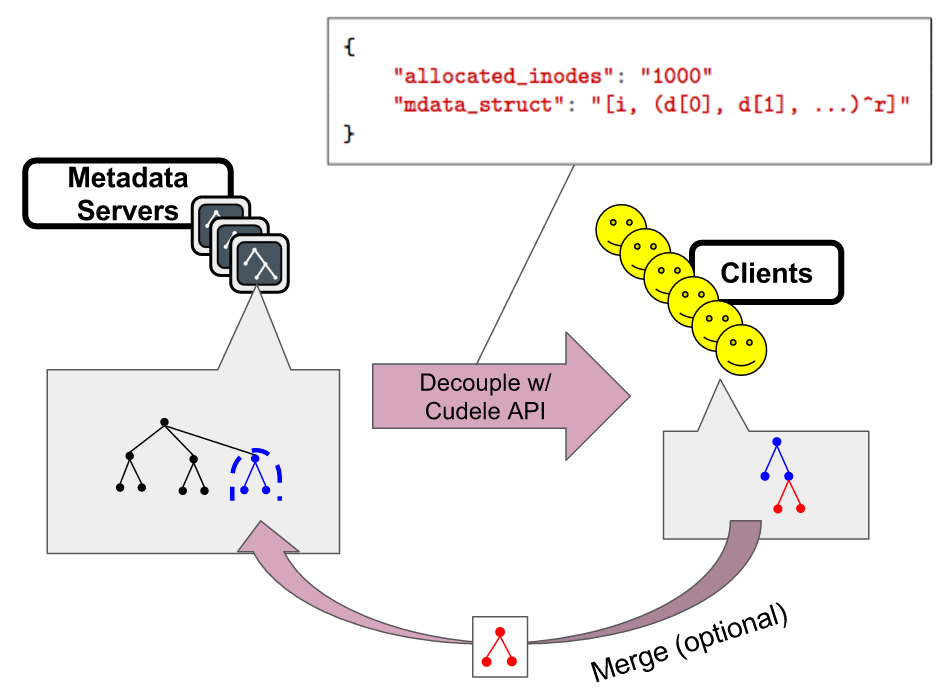
\includegraphics[width=90mm]{figures/arch.png} 
%  \caption{System XX lets clients optimize performance by telling the storage
%  system about the workload. Clients can specify a Structured Namespace (blue
%  subtrees and Section~\ref{sec:structured-namespaces}) or by merging file system
%  metadata from an Unstructured Namespace (red subtree and
%  Section~\ref{sec:unstructured-namespaces}).}\label{fig:arch}
%\end{figure}
%
%% What is Cudele
%Cudele is a file system with programmable consistency and durability. Clients
%use an API to decouple existing subtrees from the global namespace; metadata
%operations from the other clients targeted at the decoupled subtree can be
%programmed to be blocked or marked as overwritable. With the decoupled subtree
%in hand, the client can do metadata operations locally. Upon completion, the
%client can merge the subtree back into the global namespace. 
%
%% Why Cudele is a good fit for implied namespaces
%Cudele has the mechanisms for understanding the file system metadata language
%and adapting to the workload.  Figure~\ref{fig:arch} shows how clients decouple
%the namespace with the Cudele API, specifying how many extra inodes they want
%and the structure for the namespace they intend to create. The metadata server
%and client both know about the metadata in the blue subtree, requiring no RPCs,
%and if the client creates more metadata (red subtree), it can merge it back
%into the global namespace.  This model lets users enjoy the simplicity of
%global namespaces and the high performance of node-local operations.  We extend
%the API to support the declaration of structured namespaces and leverage the
%existing API to merge unstructured namespaces. 
%
%\subsubsection{Structured Namespaces}
%\label{sec:structured-namespaces}
%
%% What is a structured namespace
%A structured namespace is created according to a pattern. If both the client
%and metadata server knows the pattern, they can create the metadata
%independently. This has two benefits: (1) it reduces RPCs which improves
%performance and reduces network traffic and (2) it allows the client and server
%to operate in parallel.  The patterns that Cudele understands are shown in
%Listing~\ref{src:example} and the programmable interfaces are shown below.
%There are two parameters for unstructured namespaces: \texttt{pattern} and
%\texttt{trigger}. 
%
%\subsubsection{Trigger: Start Namespace Construction}
%
%% How does trigger work and why do we neet it
%\texttt{trigger} specifies when to start the namespace construction on the
%metadata server.  The metadata reconstruction can be asynchronous and saving
%this resource intense process for later can have better performance. To
%facilitate the exploration of different trigger policies, we make the value for
%the \texttt{trigger} parameter programmable.  Administrators inject Lua code
%that specifies or calculates thresholds for when to start namespace
%construction. Although we make this programmable, we do not make any
%conclusions about the best trigger time and leave the exploration of this space
%as future work.
%
%% example
%In Listing~\ref{src:example}, the trigger is:
%\begin{listing}
%\begin{minted}[frame=single,
%               framesep=2mm,
%               xleftmargin=10pt,
%               tabsize=2]{lua}
%{
%  if MDSs[whoami]["cpu"] > 30
%}
%\end{minted}
%\label{src:thresh}
%\end{listing}
%
%which means that construction of the namespace will start if current MDS
%(\texttt{whoami}) has a CPU utilization (\texttt{``cpu"}) above 30\%.
%
%% Drawbacks: consistency
%Triggering construction asynchronously can improve performance because the
%process can be deferred until the system has less load. However, this
%performance gain comes at the cost of consistency. Even if the construction is
%triggered immediately, the metadata is eventually consistent; other clients see
%outdated metadata because the namespace is sitting on the client. Delaying the
%trigger improves the liklihood that system finds a window of low load but also
%increases the latency of other clients.\\
%
%\noindent\emph{Implementation}: we re-use the polling and embedded Lua
%virtual machine in Mantle~\cite{sevilla:sc15-mantle} to implement the trigger
%interface. By default, every 10 seconds the metadata server checks if the
%condition for triggering is satisfied by executing the Lua code. Mantle has
%variables exposed for administrators to explore load balancing policies; just
%like this work, some of these policies need to identify overloaded metadata
%servers so we re-use all those variables.  Some of the more useful variables
%include:
%
%\begin{itemize}
%  \item Memory Usage
%  \item CPU Utilization
%  \item Request Rate
%  \item Queue Depth
%  \item Server Tags: whoami, i
%\end{itemize}
%
%\subsubsection{Pattern: Express Namespace}
%\label{sec:pattern-express-namespace}
%
%% How does pattern work and why do we need it
%\texttt{pattern} describes the metadata layout of the Structured Namespaces. It
%is the same language used in~\cite{he:hpdc13-plfs-patterns}. When the metadata
%server starts a namespace construction, it creates all the file system metadata
%generated by this formula. As a refresher, the pattern in Listing~\ref{src:example}:
%
%  \[[i, (d[0], d[1], ...)^r]\]
%
%means that there are \(r\) entries in the PLFS index file, where the first
%entry has a physical offset of \(i\) and lengths of \(d\), where the pattern in
%\(d\) repeats. \\
%
%% WTF -- this doesn't give file system metadata! ARGGGGG is it file creations
%% or index files shit?
%
%% Drawbacks
%
%\noindent\emph{Implementation}: Another big fat TODO.
%
%\begin{listing}
%\begin{minted}[frame=single,
%               framesep=2mm,
%               xleftmargin=10pt,
%               tabsize=2]{js}
%{
%  <!-- Structured Namespace Pattern !-->
%  "S_pattern": "[i, (d[0], d[1], ...)^r]",
%  
%  <!-- Structured Namespace Trigger !-->
%  "S_trigger": "if MDSs[whoami]["cpu"] > 30",
%  
%  <!-- Untructured Namespace Allocated Inos !-->
%  "US_alloci": "1000",
%}
%\end{minted}
%\caption{Using the Cudele API to express metadata structure, which is
%understood by both the server and client.}
%\label{src:example}
%\end{listing}
%
%\subsubsection{Unstructured Namespaces}
%\label{sec:unstructured-namespaces}
%
%\subsubsection{Migrating Metadata Construction}
%\label{sec:migrating-metadata-construction}
%
